%% LyX 2.3.6 created this file.  For more info, see http://www.lyx.org/.
%% Do not edit unless you really know what you are doing.
\documentclass[12pt,french]{article}
\usepackage{lmodern}
\usepackage{amsmath}
\renewcommand{\familydefault}{\rmdefault}
\usepackage[T1]{fontenc}
\usepackage[utf8]{inputenc}
\usepackage[a4paper]{geometry}
\geometry{verbose,tmargin=2cm,bmargin=2cm,lmargin=2cm,rmargin=2cm}
\usepackage{fancyhdr}
\pagestyle{fancy}
\usepackage{babel}
\makeatletter
\addto\extrasfrench{%
   \providecommand{\og}{\leavevmode\flqq~}%
   \providecommand{\fg}{\ifdim\lastskip>\z@\unskip\fi~\frqq}%
}

\makeatother
\usepackage{booktabs}
\usepackage{url}
\usepackage{amstext}
\usepackage{graphicx}
\usepackage[unicode=true,pdfusetitle,
 bookmarks=true,bookmarksnumbered=false,bookmarksopen=false,
 breaklinks=false,pdfborder={0 0 1},backref=false,colorlinks=false]
 {hyperref}

\makeatletter

%%%%%%%%%%%%%%%%%%%%%%%%%%%%%% LyX specific LaTeX commands.
%% Because html converters don't know tabularnewline
\providecommand{\tabularnewline}{\\}

%%%%%%%%%%%%%%%%%%%%%%%%%%%%%% User specified LaTeX commands.
\usepackage{listings}
\usepackage{xcolor}

\definecolor{codegreen}{rgb}{0,0.6,0}
\definecolor{codegray}{rgb}{0.5,0.5,0.5}
\definecolor{codepurple}{rgb}{0.58,0,0.82}
\definecolor{backcolour}{rgb}{0.95,0.95,0.92}

\lstdefinestyle{mystyle}{
    %backgroundcolor=\color{backcolour},   
    commentstyle=\color{codegreen},
    keywordstyle=\color{magenta},
    numberstyle=\tiny\color{codegray},
    stringstyle=\color{codepurple},
    basicstyle=\ttfamily\footnotesize,
    breakatwhitespace=false,         
    breaklines=true,                 
    captionpos=t,                    
    keepspaces=true,                 
    numbers=left,                    
    numbersep=5pt,                  
    showspaces=false,                
    showstringspaces=false,
    showtabs=false,                  
    tabsize=4
}

\lstset{style=mystyle}

\lstset{
    inputencoding = utf8,  % Input encoding
    extendedchars = true,  % Extended ASCII
    literate      =        % Support additional characters
      {á}{{\'a}}1  {é}{{\'e}}1  {í}{{\'i}}1 {ó}{{\'o}}1  {ú}{{\'u}}1
      {Á}{{\'A}}1  {É}{{\'E}}1  {Í}{{\'I}}1 {Ó}{{\'O}}1  {Ú}{{\'U}}1
      {à}{{\`a}}1  {è}{{\`e}}1  {ì}{{\`i}}1 {ò}{{\`o}}1  {ù}{{\`u}}1
      {À}{{\`A}}1  {È}{{\'E}}1  {Ì}{{\`I}}1 {Ò}{{\`O}}1  {Ù}{{\`U}}1
      {ä}{{\"a}}1  {ë}{{\"e}}1  {ï}{{\"i}}1 {ö}{{\"o}}1  {ü}{{\"u}}1
      {Ä}{{\"A}}1  {Ë}{{\"E}}1  {Ï}{{\"I}}1 {Ö}{{\"O}}1  {Ü}{{\"U}}1
      {â}{{\^a}}1  {ê}{{\^e}}1  {î}{{\^i}}1 {ô}{{\^o}}1  {û}{{\^u}}1
      {Â}{{\^A}}1  {Ê}{{\^E}}1  {Î}{{\^I}}1 {Ô}{{\^O}}1  {Û}{{\^U}}1
      {œ}{{\oe}}1  {Œ}{{\OE}}1  {æ}{{\ae}}1 {Æ}{{\AE}}1  {ß}{{\ss}}1
      {ç}{{\c c}}1 {Ç}{{\c C}}1 {ø}{{\o}}1  {Ø}{{\O}}1   {å}{{\r a}}1
      {Å}{{\r A}}1 {ã}{{\~a}}1  {õ}{{\~o}}1 {Ã}{{\~A}}1  {Õ}{{\~O}}1
      {ñ}{{\~n}}1  {Ñ}{{\~N}}1  {¿}{{?`}}1  {¡}{{!`}}1
      {°}{{\textdegree}}1 {º}{{\textordmasculine}}1 {ª}{{\textordfeminine}}1
      % ¿ and ¡ are not correctly displayed if inconsolata font is used
      % together with the lstlisting environment. Consider typing code in
      % external files and using \lstinputlisting to display them instead.      
  }


\@ifundefined{showcaptionsetup}{}{%
 \PassOptionsToPackage{caption=false}{subfig}}
\usepackage{subfig}
\makeatother

\begin{document}

\lhead{Sorbonne Université, UE LU3PY126 FOAD, 2023}

\rhead{PUJOL Martin}
\title{Projet Dynamique Quantique}
\author{PUJOL Martin}

\maketitle
\tableofcontents{}

\clearpage{}

\section{Introduction}

La possibilité de décrire l'évolution temporelle d'un système quantique, c'est-à-dire l'évolution au cours du temps de sa fonction d'onde $\Psi(\vec{r}, t)$, est un des résultats majeurs de la physique quantique. La mécanique quantique est une théorie fondamentale de la physique qui a connu un développement considérable au cours du XXe siècle, avec de nombreuses applications en physique, chimie, biologie, informatique, etc. Les équations de Schrödinger décrivent l'évolution des systèmes quantiques et leur résolution numérique est un enjeu important en physique théorique et en simulation numérique.

La résolution numérique des équations de Schrödinger dépendantes du temps est un défi qui nécessite des méthodes numériques adaptées, que ce soit pour des systèmes unidimensionnels ou multidimensionnels. Ces méthodes font appel à des algorithmes de calcul intensif qui nécessitent des ressources informatiques importantes. La puissance de calcul est donc une ressource limitée et au cœur de notre étude.

Dans ce projet, nous allons mettre en œuvre des méthodes numériques pour résoudre l'équation de Schrödinger dépendante du temps pour une particule de masse $m$ soumise à l'action d'un potentiel unidimensionnel $V(x)$. Cette équation décrit l'évolution temporelle de la fonction d'onde $\Psi(x,t)$ de la particule et est donnée par l'équation (3). Le potentiel unidimensionnel peut être utilisé pour modéliser différents systèmes, tels que des particules dans un puits de potentiel, des électrons dans un cristal, des atomes dans un gaz ou même des molécules dans un milieu environnant.

Nous allons d'abord étudier les états stationnaires du système, qui correspondent aux solutions indépendantes du temps de l'équation de Schrödinger. Ces états stationnaires sont très importants en physique quantique car ils permettent de déterminer les propriétés fondamentales du système, telles que les niveaux d'énergie et les fonctions d'onde associées. Pour ce faire, nous allons utiliser la méthode des moindres carrés pour résoudre l'équation de Schrödinger dans le domaine discret en remplaçant les dérivées partielles par des différences finies. Nous allons également utiliser des méthodes d'intégration numérique pour calculer les valeurs propres et les vecteurs propres associés de la matrice représentant le hamiltonien du système.

Ensuite, nous allons étudier l'évolution temporelle du système en utilisant des méthodes numériques d'intégration, telles que la méthode d'Euler et la méthode de Runge-Kutta d'ordre 4 (RK4). Ces méthodes permettent de calculer la fonction d'onde $\Psi(x,t)$ à différents instants $t$, en utilisant la fonction d'onde à l'instant initial $t=0$ comme condition initiale. Nous allons également utiliser des méthodes d'analyse numérique pour étudier la convergence et la stabilité de ces méthodes d'intégration.

Enfin, nous allons comparer les résultats numériques avec les résultats analytiques pour des systèmes simples ce qui nous permettra de conclure quant à l'importance la discrétisation de l'espace et du temps.


\section{Matériel et Méthodes}

\subsection{ Méthodes de résolution : Partie 1}

Dans un premier temps, on souhaite determiner les états propres de l'hamiltonien, rappelons son expression : 


$$-\frac{\hbar^2}{2m}\frac{d^2\psi}{dx^2} + V(x)\psi = E\psi$$

où $\hbar$ est la constante de Planck réduite, $m$ est la masse de la particule, $V(x)$ est le potentiel, $E$ est l'énergie propre de l'état stationnaire $\psi$.

Nous cherchons à résoudre cette équation pour trouver les valeurs propres de l'Hamiltonien. Pour cela, nous pouvons discrétiser l'espace en utilisant une méthode de différences finies. En discrétisant l'espace, nous remplaçons la dérivée seconde par une différence finie centrée, de sorte que l'équation devient :

$$-\frac{\hbar^2}{2m}\frac{\psi_{i+1}-2\psi_i+\psi_{i-1}}{\Delta x^2} + V_i\psi_i = E\psi_i$$

où $i$ est l'indice discret de la position le long de la direction $x$, et $\Delta x$ est la distance entre les points discrets. On peut écrire cette équation sous forme matricielle :

$$\mathbf{H}\mathbf{\psi} = E\mathbf{\psi}$$

où $\mathbf{H}$ est la matrice de l'Hamiltonien, $\mathbf{\psi}$ est le vecteur d'onde discrétisé, et $E$ est l'énergie propre discrétisée.

En utilisant la méthode de la différence finie, la matrice $\mathbf{H}$ devient une matrice tridiagonale, avec des éléments diagonaux et hors-diagonaux spécifiques. La diagonale principale est donnée par :

$$\mathbf{H}_{ii} = \frac{\hbar^2}{m\Delta x^2} + V_i$$

et les termes hors diagonale sont :

$$\mathbf{H}_{i,i+1} = \mathbf{H}_{i+1,i} = -\frac{\hbar^2}{2m\Delta x^2}$$

Ensuite, pour trouver les valeurs propres de la matrice de l'Hamiltonien, nous utiliserons la méthode de la diagonalisation tridiagonale. 

En utilisant cette méthode, nous pouvons diagonaliser la matrice de l'Hamiltonien pour trouver les valeurs propres discrètes et les vecteurs propres associés. Ces valeurs propres et vecteurs propres correspondent aux énergies propres et fonctions d'onde discrétisées respectivement.

En résumé, la méthode de la différence finie nous permet de discrétiser l'équation d'onde stationnaire pour trouver les fonctions d'ondes propres de l'hamiltonien (aussi discrétisées).

\subsection{ Méthodes de résolution : Partie 2}

Dans la partie 2, nous avons étudié l'évolution temporelle de la fonction d'onde d'une particule dans un potentiel unidimensionnel en résolvant l'équation de Schrödinger dépendante du temps, donnée par :

$$i\hbar\frac{\partial}{\partial t}\Psi(x,t) = \hat{H}\Psi(x,t)$$

où $\hbar$ est la constante de Planck réduite et $\hat{H}$ est l'opérateur hamiltonien du système. Pour trouver une relation différentielle pour la fonction d'onde $\Psi(x,t)$, nous avons utilisé l'opérateur hamiltonien de la particule dans un potentiel unidimensionnel :

$$\hat{H} = -\frac{\hbar^2}{2m}\frac{\partial^2}{\partial x^2} + V(x)$$

où $m$ est la masse de la particule et $V(x)$ est le potentiel unidimensionnel.

En substituant l'opérateur hamiltonien dans l'équation de Schrödinger, nous avons obtenu l'équation suivante :

$$i\hbar\frac{\partial}{\partial t}\Psi(x,t) = -\frac{\hbar^2}{2m}\frac{\partial^2}{\partial x^2}\Psi(x,t) + V(x)\Psi(x,t)$$

Nous avons ensuite discrétisé l'espace en remplaçant la fonction d'onde continue par des valeurs discrètes $\Psi_j^n$, où $j$ représente la position spatiale et $n$ représente le temps. Nous avons également remplacé les dérivées partielles par des différences finies pour obtenir une relation de récurrence pour les valeurs discrètes de la fonction d'onde :

$$i\hbar\frac{\Psi_j^{n+1}-\Psi_j^{n}}{\Delta t} = -\frac{\hbar^2}{2m}\frac{\Psi_{j+1}^{n}-2\Psi_j^{n}+\Psi_{j-1}^{n}}{\Delta x^2} + V_j\Psi_j^{n}$$

où $\Delta x$ et $\Delta t$ sont les pas de discrétisation pour l'espace et le temps, respectivement, et $V_j$ est la valeur du potentiel en la position $j\Delta x$. Cette relation de récurrence est appelée la méthode d'Euler explicite pour résoudre l'équation de Schrödinger dépendante du temps.

Nous pouvons également utiliser des méthodes d'intégration numérique plus précises pour résoudre cette équation, telles que la méthode de Runge-Kutta d'ordre 4 (RK4). Dans ce cas, nous obtenons une relation de récurrence plus complexe pour les valeurs discrètes de la fonction d'onde, qui implique des calculs supplémentaires à chaque étape de temps.

En conclusion, pour résoudre l'équation de Schrödinger dépendante du temps pour une particule dans un potentiel unidimensionnel, nous avons discrétisé l'espace en utilisant des différences finies et résolu la relation de récurrence obtenue en utilisant des méthodes d'intégration numérique, telles que la méthode d'Euler ou la méthode de RK4.





\subsection{Les outils python}

Dans ce projet, différentes librairies Python ont été utilisées pour simuler la dynamique d'un paquet d'onde gaussien dans différents potentiels. Tout d'abord, la librairie NumPy a été utilisée pour manipuler des tableaux multidimensionnels, ce qui a permis d'effectuer des calculs vectoriels efficaces et d'optimiser les performances.

Ensuite, la librairie Matplotlib a été utilisée pour créer des graphiques et des animations. Matplotlib.pyplot a permis de tracer les graphes de l'évolution temporelle de la fonction d'onde et de la position moyenne de la particule associée. Quant à Matplotlib.animation, elle a été utilisée pour créer les animations correspondantes.

La librairie Numba a également été utilisée pour optimiser les performances des calculs. 

En résumé, ces différentes librairies ont permis de réaliser une simulation efficace et précise de la dynamique de fonctions d'onde dans différents potentiels, en combinant les avantages de l'optimisation de code, de la visualisation graphique et de la résolution numérique d'équations différentielles.

\subsection{Les codes python (voir annexe)}

Le programme principale de la première partie est "resol.py".
Ce programme permet de résoudre l'équation d'onde en discrétisant l'espace en n points, avec une taille totale de L. La fonction resol prend en entrée la longueur totale L, le nombre de points n, le potentiel et un paramètre booléen Norm qui indique si l'on souhaite normaliser la fonction d'onde. La fonction calcule les valeurs propres w et les vecteurs propres v de la matrice tridiagonale associée à l'équation d'onde discrétisée et renvoie les résultats sous forme de tableaux numpy.Ensuite, la fonction normalize permet de normaliser les vecteurs propres si le paramètre Norm est True.
\newline 

Les fonctions correspondant aux potentiels sont stockés dans "potentiels.py".
\newline

"potentiel stationnaire quantitatif.py" est un programme en Python qui permet d'apprécier la résolution numérique de l'équation de Schrödinger pour différents potentiels usuels, et de retrouver les résultats habituels de la quantification de l'énergie et des formes souvent sinusoidales des fonctions d'onde.

Il utilise des modules de calculs et de visualisation tels que matplotlib et des fonctions spécifiques pour résoudre l'équation de Schrödinger pour différents potentiels tels que le puit de potentiel, la barrière de potentiel, le double puits de potentiel, le potentiel périodique, etc. Le programme utilise des paramètres de simulation pour déterminer les fonctions d'onde et les énergies propres des systèmes.
Pour chaque potentiel, il trace les 10 premières fonctions d'ondes, représentant la densité de probabilité de présence et l'énergie propre de chaque fonction d'onde. Les résultats sont enregistrés sous forme de fichiers image pour chaque potentiel.

\newline

Pour la deuxième partie, il est d'abord nécessaire d'implémenter les deux méthodes numériques qui nous permettront de résoudre l'évolution temporelle de la fonction d'onde.

D'abord, le programme "euler.py" contient plusieurs fonctions. La première est "euler", qui implémente la méthode d'Euler pour résoudre une équation différentielle. Cette fonction prend en entrée une fonction f, les bornes a et b de l'intervalle sur lequel on veut résoudre l'équation, le nombre N de pas de discrétisation, la condition initiale y0 et un éventuel vecteur de paramètres. La fonction retourne un tableau des N valeurs prises par y avec un pas h. La méthode d'Euler est une méthode numérique simple pour résoudre des équations différentielles. Elle consiste à estimer la valeur de la fonction à chaque pas h en utilisant sa valeur et sa dérivée à l'instant courant.

La seconde fonction dans "euler.py" est "normalize", qui prend une matrice en entrée et la normalise en colonnes en divisant chaque colonne par sa norme. Elle divise ensuite la matrice par la racine carrée du pas de discrétisation. Cette fonction s'assure que la somme des probabilitées de présence sont bien égales à 1.

\newline

La seconde méthode numérique implémenté est la méthode de Runge Kutta d'ordre 4. Pour se faire, le programme "rk4.py" commence par définir une fonction "rk4" qui prend en entrée le pas de temps, les valeurs de la fonction au temps t(i), une fonction dérivée et les paramètres, et qui renvoie les nouvelles valeurs de la fonction pour t(i+1) en utilisant la méthode de Runge-Kutta d'ordre 4.

Ensuite, le programme définit une fonction "RK4" qui prend en entrée une fonction dérivée, une borne inférieure a, une borne supérieure b, le nombre de points N, la valeur initiale de la fonction y0 et les paramètres, et qui renvoie un tableau de N valeurs de la fonction en utilisant la méthode de Runge-Kutta d'ordre 4.

\newline
Ces  deux méthodes étant définis, il est nécéssaire de introduire la fonction traduisant l'évolution temporelle d'une fonction d'onde.
La fonction "deriv" calcule donc la dérivée de la fonction d'onde "y" en utilisant la méthode de différences finies. 
\newline 
Les programmes "evolution RK4.py" et "evolution euler.py" permettent d'apprecier la qualité de respective de ces méthodes.
Le programme enregistre ensuite quelques valeurs et trace l'évolution de l'erreur sur l'état stationnaire pour plusieurs valeurs de delta t. Les erreurs sont calculées pour les valeurs de delta_t = 1e-2, 1e-3 et 1e-4, et sont enregistrées dans "error1", "error2" et "error3", respectivement. Les temps correspondants sont stockés dans les tableaux "temps1", "temps2" et "temps3".

Finalement, le programme trace l'évolution de l'erreur sur l'état stationnaire pour les trois valeurs de delta t. Ces graphiques sont enregistrés dans "RK4_Precision.png".

\newline
Enfin, plusieurs programmes ont été créé afin de mettre en évidence la dynamique d'un paquet d'onde gaussien dans différents potentiels.Chacun de ces programmes comprend une animation ainsi que 10 graphes qui retracent l'évolution temporelle de la fonction d'onde. Les graphes tracent également la position moyenne de la particule associée à la fonction d'onde. Cette simulation peut être utile pour visualiser et comprendre le comportement des paquets d'ondes dans différents environnements potentiels.


\clearpage{}

\section{Résultats}


\subsection{Partie une}
\begin{figure}[htbp]
\centering
\begin{minipage}[b]{0.45\linewidth}
\centering
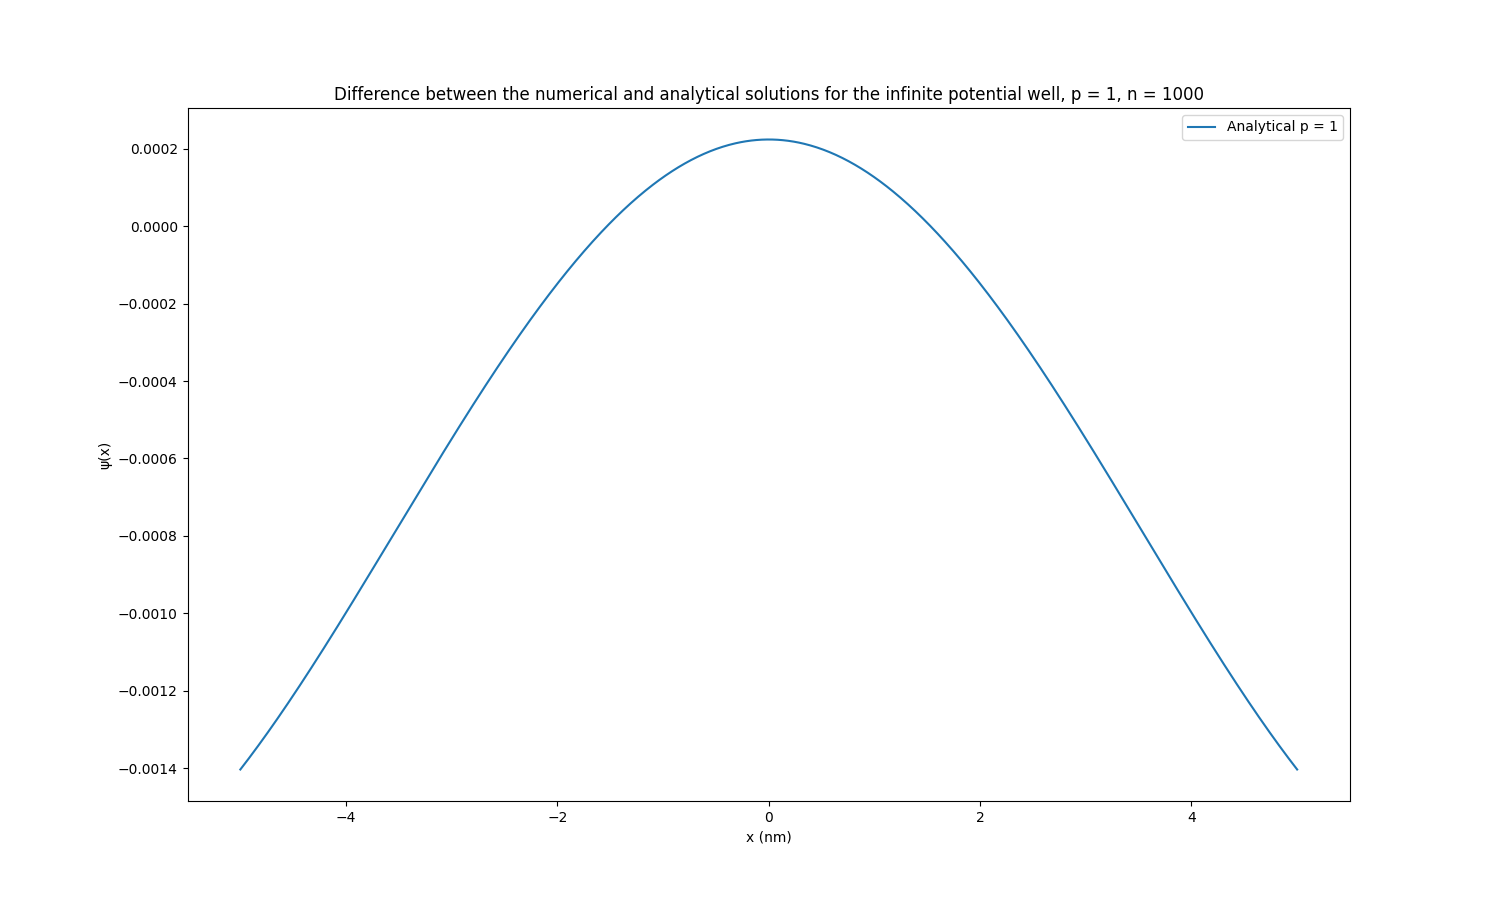
\includegraphics[width=\linewidth]{Partie_I/PartieI_puit_infini_n1000.png}
\caption{Erreur pour delta_t = 1e-2}
\label{fig:puit-infini}
\end{minipage}
\hfill
\begin{minipage}[b]{0.45\linewidth}
\centering
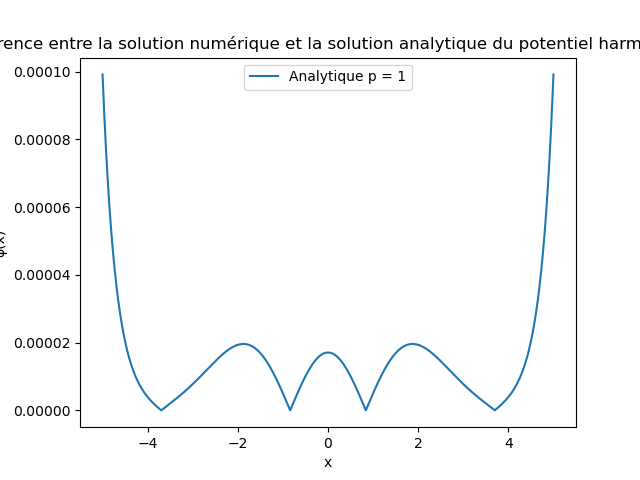
\includegraphics[width=\linewidth]{Partie_I/PartieI_potentiel_harmonique_n10000.png}
\caption{Erreur pour delta_t = 1e-3}
\label{fig:potentiel-harmonique}
\end{minipage}
\end{figure}
Dans un premier temps, notre objectif était de trouver la valeur optimale pour delta t. Bien que l'on s'attende à ce qu'une valeur de delta t plus faible réduise l'erreur, il était également important de limiter le temps de calcul pour que les simulations restent réalisables.
Ci-dessus, on peut observer un graphique représentant l'erreur pour des valeurs de delta t de 1e-2 et 1e-3.

\clearpage

\begin{figure}[htbp]
\centering
\begin{minipage}[b]{0.45\linewidth}
\centering
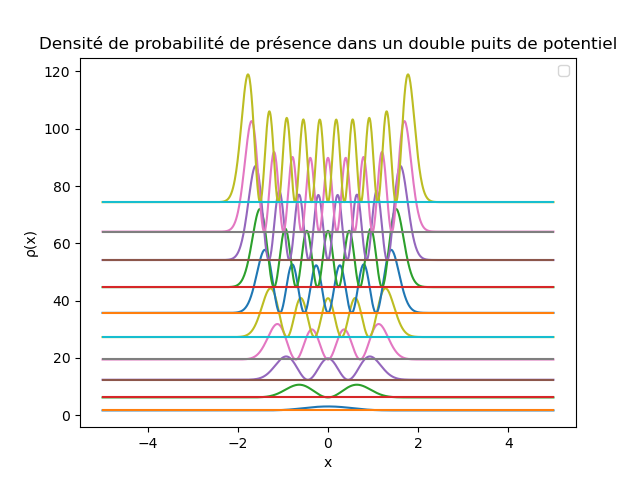
\includegraphics[width=\linewidth]{Partie_I/Double_puits_de_potentiel.png}
\caption{Double puits de potentiel}
\label{fig:double-puit}
\end{minipage}
\hfill
\begin{minipage}[b]{0.45\linewidth}
\centering
\includegraphics[width=\linewidth]{Partie_I/Barrière_de_potentiel_amortie.png}
\caption{Barrière de potentiel amortie}
\label{fig:barriere-potentiel}
\end{minipage}
\caption{Graphiques de différents potentiels}
\label{fig:potentiels2}
\centering
\begin{minipage}[b]{0.45\linewidth}
\centering
\includegraphics[width=\linewidth]{Partie_I/Potentiel_périodique.png}
\caption{Potentiel périodique}
\label{fig:double-puit}
\end{minipage}
\hfill
\begin{minipage}[b]{0.45\linewidth}
\centering
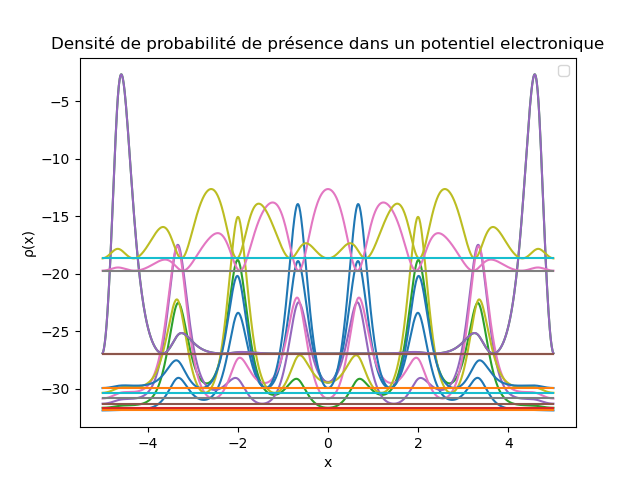
\includegraphics[width=\linewidth]{Partie_I/Potentiel_electronique.png}
\caption{Potentiel electronique}
\label{fig:barriere-potentiel}
\end{minipage}

\end{figure}

Les graphiques 3 à 7 nous permettent d'apprécier la résolution des fonctions d'onde propres pour différents potentiels tels que les doubles puits, les barrières de potentiel amorties, les potentiels périodiques et les potentiels électroniques. Les densités de probabilité de présence présentent des formes très satisfaisantes, rappelant des formes fréquentes en physique. Nous pouvons également remarquer la conservation des propriétés de symétrie du système ainsi que la quantification des niveaux d'énergie. Sur ces graphiques, nous avons ainsi 10 densités de probabilité de présence décalées par leurs énergies propres.

\clearpage{}


\subsection{Partie deux}
Tout d'abord, il était nécessaire de déterminer les valeurs optimales de delta t et de delta x pour les simulations. Pour réduire la discrétisation en x, une valeur minimale de delta x de 0.1 a été choisie pour un intervalle de longueur 10. Cette limite était nécessaire car les calculs sont répétés à chaque itération. En considérant l'équation différentielle, il était prévu que le rapport delta t / (delta x)**2 ne soit pas trop grand. Afin de confirmer cette hypothèse, un graphique de l'erreur dans le temps a été tracé pour trois valeurs de delta t.


\begin{figure}[htbp]
\centering
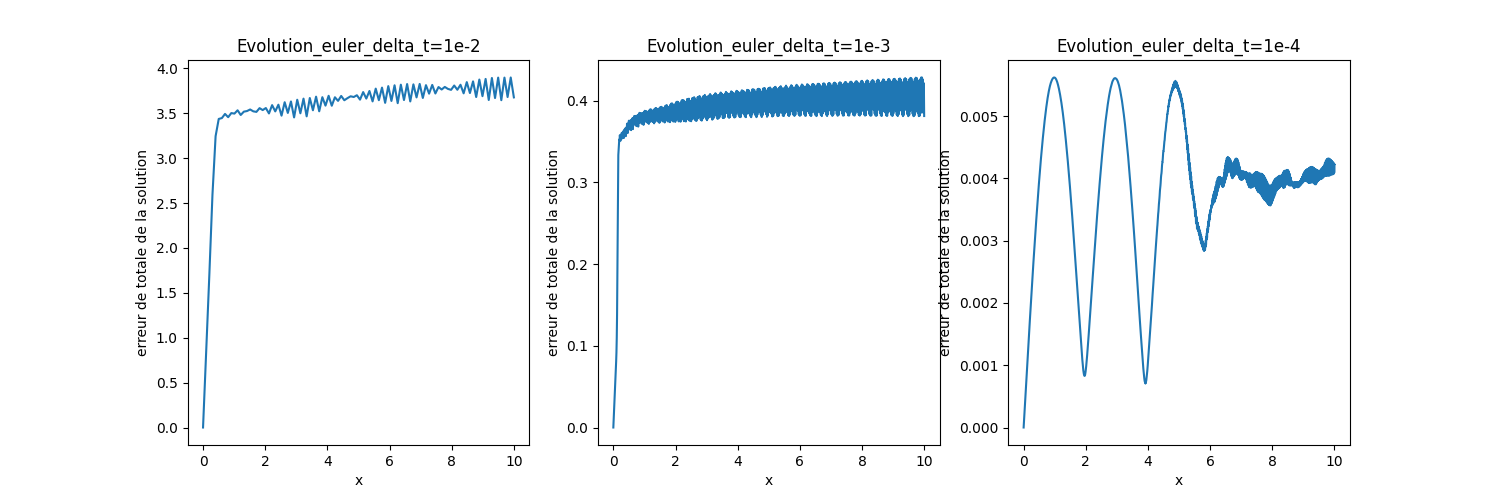
\includegraphics[width=0.7\linewidth]{Partie_II/Euler_Precision.png}
\caption{Evolution de l'erreur de la méthode d'Euler}

\centering
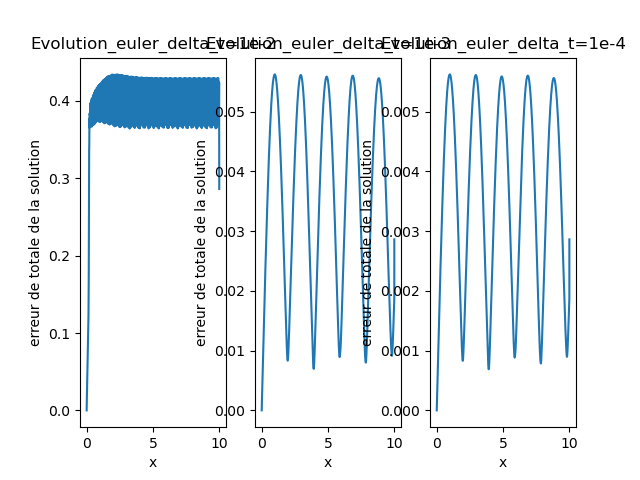
\includegraphics[width=0.7\linewidth]{Partie_II/RK4_Precision.png}
\caption{Evolution de l'erreur de la méthode de Runge-Kutta 4}
\end{figure}

Les graphes suivants présentent l'évolution de l'erreur de la méthode d'Euler et de la méthode de Runge-Kutta 4 (RK4) en fonction du temps pour différentes valeurs de delta t. On peut voir que pour une valeur de delta t trop grande, l'erreur augmente rapidement, tandis que pour une valeur de delta t suffisamment petite, l'erreur reste faible et stable. En général, la méthode de RK4 est plus précise que la méthode d'Euler pour toutes les valeurs de delta t testées. On choisira donc de poursuivre les simulations avec la méthode de RK4 et delta t = 10000.

\begin{figure}[htbp]
\centering
\begin{minipage}[b]{0.45\linewidth}
\centering
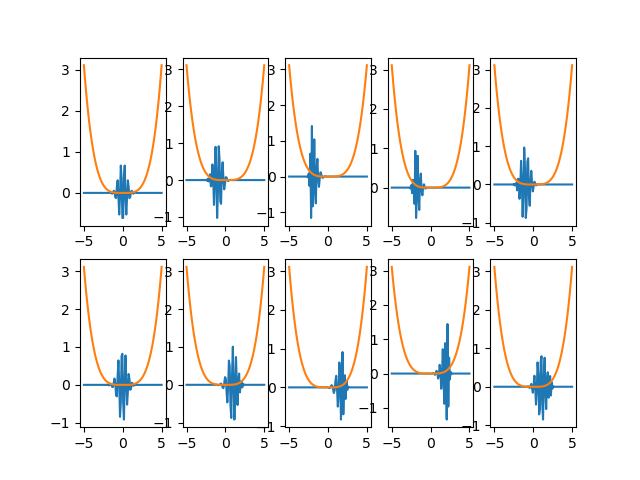
\includegraphics[width=\linewidth]{Partie_II/Dynamique_Paquet_Onde_Potentiel_Harmonique.png}
\caption{Dynamique d'un paquet d'onde dans un potentiel harmonique}
\label{fig:double-puit}
\end{minipage}
\hfill
\begin{minipage}[b]{0.45\linewidth}
\centering
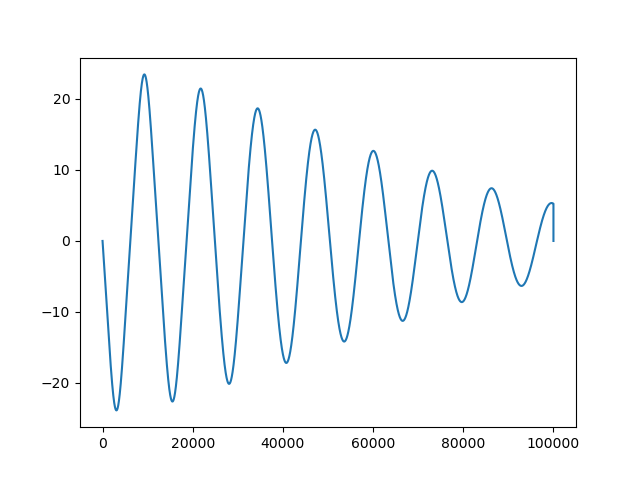
\includegraphics[width=\linewidth]{Partie_II/Position_Moyenne_Paquet_Onde_Potentiel_Harmonique.png}
\caption{Position moyenne de la particule associée}
\label{fig:barriere-potentiel}
\end{minipage}
\end{figure}

La figure 10 illustre l'oscillation du paquet d'ondes dans un potentiel harmonique. Afin d'obtenir une évolution significative du déplacement, l'onde possède une énergie très élevée (k0 = 1e10). Cependant, malgré cette énergie élevée, on observe un étalement de la position au fil du temps, qui peut également être associé aux erreurs de la méthode. Par ailleurs, la position moyenne de la particule présente un comportement très intéressant : elle oscille périodiquement tout en semblant converger vers 0.
La dynamique d'une particule dans un potentiel harmonique suit une oscillation périodique classique. Cette observation permet de caractériser l'état quasi-classique de la particule.

\clearpage{}
Les figures 12 et 13 sont des extensions des simulations précédentes où un paquet d'onde associé à une particule traverse un potentiel composé de 6 électrons uniformément répartis. On peut observer que le paquet d'onde semble piégé au centre où le potentiel est plus élevé. Le graphe 13 représente le même potentiel que le graphe 12, mais avec une énergie plus élevée pour chaque électron.

\begin{figure}[htbp]
\centering
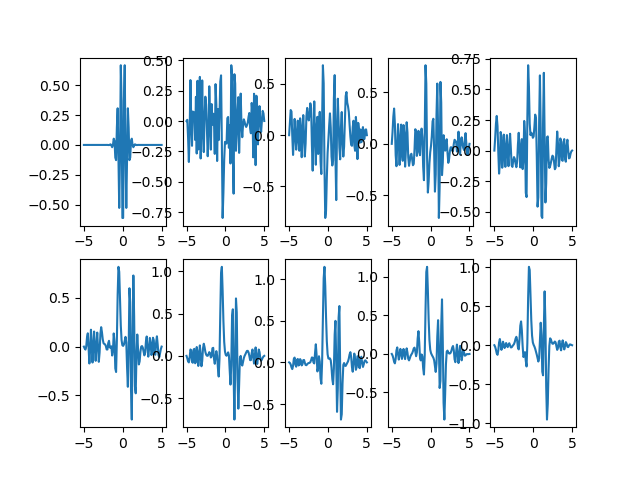
\includegraphics[width=0.5\linewidth]{Partie_II/Dynamique_Paquet_Onde_Potentiel_Electronique_potentiel_plus_bas.png}
\caption{Dynamique d'un paquet d'onde dans un potentiel electronique}
\label{fig:double-puit}
\end{figure}
\begin{figure}[htbp]
\centering
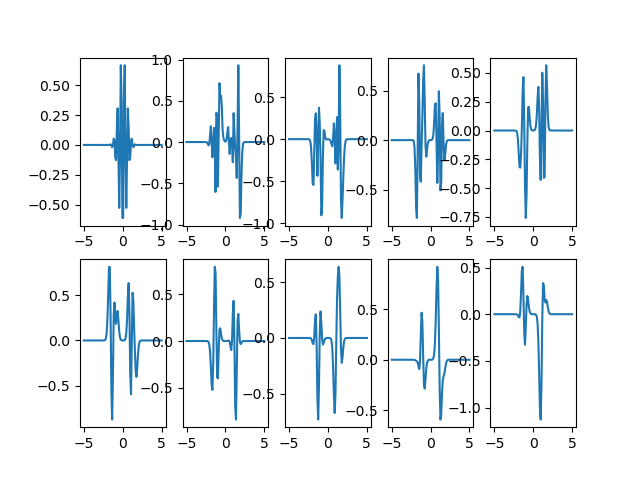
\includegraphics[width=0.5\linewidth]{Partie_II/Dynamique_Paquet_Onde_Potentiel_Electronique.png}
\caption{Dynamique d'un paquet d'onde dans un potentiel electronique plus faible}
\label{fig:barriere-potentiel}

\end{figure}



\clearpage{}







\section{Discussion des résultats}

Dans un premier temps, on peut orienter notre discussion sur les méthodes de résolutions numérique : 
La première partie de l'étude consistait à résoudre les états propres de l'Hamiltonien pour différents potentiels. Le premier objectif était de déterminer la valeur optimale de delta t qui minimise l'erreur tout en limitant le temps de calcul. Les graphiques représentant l'erreur pour des valeurs de delta t de 1e-2 et 1e-3 montrent une nette réduction de l'erreur pour une valeur de delta t plus faible, mais avec une augmentation significative du temps de calcul. Il a donc été décidé d'utiliser une valeur de delta t de 1e-3, qui donnait une erreur raisonnable tout en conservant un temps de calcul raisonnable.

Les graphes suivants présentaient la résolution des fonctions d'onde propres pour différents potentiels. Les densités de probabilité de présence obtenues sont très satisfaisantes, présentant des formes correspondant aux propriétés physiques attendues pour chaque potentiel, tout en respectant la conservation des propriétés de symétrie du système et la quantification des niveaux d'énergie.

Dans la deuxième partie de l'étude, nous avons examiné l'évolution d'une fonction d'onde dans le temps. Les valeurs optimales de delta t et de delta x ont été déterminées en fonction de l'équation différentielle à résoudre, en s'assurant que le rapport delta t / (delta x)**2 ne soit pas trop grand. Les graphes montrant l'évolution de l'erreur pour différentes valeurs de delta t ont confirmé cette hypothèse.

Les graphes représentant l'évolution de l'erreur de la méthode d'Euler et de la méthode de Runge-Kutta 4 montrent une réduction significative de l'erreur avec l'utilisation de la méthode de Runge-Kutta 4. Cette méthode offre une précision nettement supérieure pour la même valeur de delta t. Cependant, le temps de calcul pour la méthode de Runge-Kutta 4 est considérablement plus long que celui de la méthode d'Euler.


En ce qui concerne les résultats eux-mêmes, nous avons tout d'abord été soulagés de constater que les niveaux d'énergie étaient quantifiés, et que les solutions analytiques prédites pour les premiers niveaux d'énergie du puits de potentiel carré infini et du potentiel harmonique étaient correctes. Nous avons également apprécié les différentes formes de densités de probabilité. L'élément majeur qui a confirmé l'exactitude de ces calculs a été le fait que les fonctions d'onde n'évoluent pas dans le temps, contrairement à leurs combinaisons linéaires ou à un paquet d'onde.

Enfin, en ce qui concerne la dynamique des fonctions d'onde, après avoir montré des résultats simples ou attendus, nous nous sommes intéressés à leur dynamique. Nous avons pu observer comment un paquet d'onde gaussien oscillait périodiquement dans un potentiel harmonique, ce qui nous a amené à la notion d'état quasi-classique. Un résultat intéressant a également été de constater comment une particule peut être piégée par un ou plusieurs électrons. Dans notre cas, la fonction d'onde s'est retrouvée confinée dans les deux électrons au centre (où le potentiel est le plus élevé) avec une probabilité oscillant de l'un à l'autre.
\section{Conclusion}

Ce projet de a permis de mettre en place des méthodes de résolution numérique pour l'équation de Schrödinger dépendante du temps, en se basant sur l'Hamiltonien du système. Les résultats obtenus ont montré que les valeurs optimales de delta t et delta x ont été déterminées en fonction de l'équation différentielle à résoudre, en s'assurant que le rapport delta t / (delta x)**2 ne soit pas trop grand. Les graphes montrant l'évolution de l'erreur pour différentes valeurs de delta t ont confirmé cette hypothèse.

Les graphiques ont également montré que la méthode de Runge-Kutta 4 offrait une précision nettement supérieure pour la même valeur de delta t par rapport à la méthode d'Euler, mais le temps de calcul pour la méthode de Runge-Kutta 4 est considérablement plus long. En ce qui concerne les résultats eux-mêmes, les niveaux d'énergie étaient quantifiés, et les solutions analytiques prédites pour les premiers niveaux d'énergie du puits de potentiel carré infini et du potentiel harmonique étaient correctes. Les différentes formes de densités de probabilité ont également été appréciées.

Le projet a également permis d'observer la dynamique d'un paquet d'onde gaussien oscillant périodiquement dans un potentiel harmonique, amenant à la notion d'état quasi-classique, et comment une particule peut être piégée par un ou plusieurs électrons. Dans le cas étudié, la fonction d'onde s'est retrouvée confinée dans les deux électrons au centre (où le potentiel est le plus élevé) avec une probabilité oscillant de l'un à l'autre.

En conclusion, le projet a permis de comprendre et d'appliquer les méthodes numériques pour la résolution de l'équation de Schrödinger dépendante du temps et de mettre en évidence les propriétés quantiques d'un système. Le potentiel harmonique et le puits de potentiel carré infini ont été étudiés, montrant l'exactitude des calculs à travers la quantification des niveaux d'énergie et la conservation des propriétés de symétrie du système. Les résultats obtenus ont montré la possibilité de décrire l'évolution temporelle d'un système quantique, ainsi que sa dynamique et ses propriétés.

\clearpage{}



\bibliographystyle{unsrt}
\bibliography{biblio}

\clearpage{}

\section{Annexe}

Si besoin, pour mettre des figures supplémentaires, mais moins importantes.
Ou encore les codes python.

\subsection{Codes python}

Sous LyX on peut importer un code via le menu \og Insert->File->Child
Document\fg , comme c'est fait ici:

\lstinputlisting[language=Python,caption={},label {}]{Partie_I/resol.py}
\lstinputlisting[language=Python,caption={},label {}]{Partie_I/potentiels.py}
%\lstinputlisting[language=Python,caption={},label {}]{Partie_I/potentiels_stationnaires_quantitatifs.py}
%\lstinputlisting[language=Python,caption={},label {}]{Partie_I/potentiels_stationnaires_qualitatifs.py}
\lstinputlisting[language=Python,caption={},label {}]{Partie_II/deriv.py}
\lstinputlisting[language=Python,caption={},label {}]{Partie_II/euler.py}
\lstinputlisting[language=Python,caption={},label {}]{Partie_II/rk4.py}
\lstinputlisting[language=Python,caption={},label {}]{Partie_II/evolution_euler.py}
\lstinputlisting[language=Python,caption={},label {}]{Partie_II/evolution_rk4.py}
\lstinputlisting[language=Python,caption={},label {}]{Partie_II/paquet_onde_potentiel_harmonique.py}
%\lstinputlisting[language=Python,caption={},label {}]{Partie_I/paquet_onde_puit_de_potentiel.py}


LyX utilise le paquet LaTeX \og listings\fg{} pour cela, avec la commande
\og\textbackslash lstinputlisting\fg . On peut changer le style
d'affichage dans le menu \og Document->Settings->LaTeX Preamble\fg{}
où on peut mettre du code LaTeX pour configurer les \og listings\fg .
Le style est adapté de cette source:

\url{https://www.overleaf.com/learn/latex/Code_listing}

\lstinputlisting[language=Python,caption={},label={}]{}
\end{document}
